%\documentclass[amsmath,amssymb,11pt]{article}
%\usepackage{graphicx}
%\usepackage{caption} 
%\usepackage{xcolor}
%\renewcommand{\thesection}{\Roman{section}} 
%\renewcommand{\thesubsection}{\Roman{subsection}}
%\pagestyle{empty}
%ADJUSTING MARGINS

%\addtolength{\oddsidemargin}{-.5in}
%\addtolength{\evensidemargin}{-.5in}
%\addtolength{\textwidth}{1in}
%\addtolength{\topmargin}{-1.5cm}
%\addtolength{\textheight}{1.5in}

%\footskip{.5in}
%\addtolength{\bmargin}{-.7in}


%\begin{document}
\begin{center}
{\Large \textcolor{red}{\bf MOCVD}}\\
\end{center}
\setlength{\fboxrule}{1pt}%
\framebox{\makebox[\textwidth][r]{\colorbox{cyan!40}{\parbox[l]{15cm}{\large{\bf Name: Vatsala Swaroop} \\ {\bf Roll No: BT12ECE086} \hfill {\framebox{
\includegraphics[height=3.5cm]{vnitlogo.png}}}}}}}
\begin{flushleft}
\vspace{5mm}
\section{Introduction}
\vspace{2mm}
The fabrication of the quantum devices is an outstanding challenge in nanostructure materials science.This assignment is an attempt to understand Metal-Organic Chemical Vapour Deposition (MOCVD),one of the most widely used epitaxial technologies to manufacture electronic devices.
\vspace{3mm}
\newline
Over the years,this approach was chosen over other methods because of its flexibility in growing precision controlled layers for special applications as well as it's ability to be scaled up to industrial-scale production with relative ease.Many industries have come up with their own setup and reactors to use this technique for their products.
\vspace{5mm}
\newline
\begin{figure}[h!] 
	\centering
	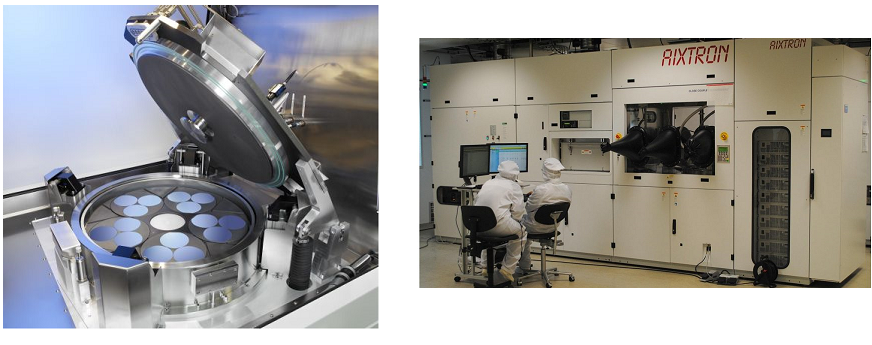
\includegraphics[width=15cm, height=8cm]{images/axitron.png} 
	\caption{Mocvd Reactor built by one such industry-Aixtron}
	\label{fig:img1} 
\end{figure} 
\vspace{3mm}
\newline
MOCVD is also known as: MOVPE (metal organic vapor phase epitaxy), OMVPE (organo-metallic vapor phase epitaxy) and OMCVD (organo-metallic chemical vapor deposition).
\vspace{1mm}
\section{Definitions/ Principle of Operation}
\vspace{2mm}
\textbf{What is MOCVD?}
\vspace{3mm}
\newline
MOCVD is a process for growing crystalline layers.It is a technique that is used to deposit very thin layers of atoms onto a semiconductor wafer.It uses the CVD(chemical vapor deposition) method,wherein gases containing the required chemical elements are made to react in the vicinity of the substrate inside the reactor.The required chemical elements in this case are organometallic and hydrides precursors accompanied by carrier gases and hence,the term metal-organic is used.
\vspace{3mm}
\newline
\large{{\textit{Key terms} :-}}\\*
\vspace{3mm}
A \textbf{precursor} is a compound that participates in the chemical reaction that produces another compound
\vspace{3mm}
\newline
\textbf{Epitaxy} is the deposition of thin, single layers on a suitable substrate on which they grow in the form of crystals. The word stems from the Greek term  meaning stacked or arranged in layer. 
\vspace{5mm}
\newline
\begin{figure}[h!] 
	\centering
	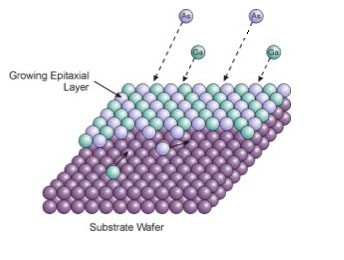
\includegraphics[width=8cm, height=6cm]{images/epitaxy.png} 
	\caption{Epitaxial growth involving Ga and As atoms}
	\label{fig:img2} 
\end{figure} 
\vspace{6mm}
\newline
\textbf{Working Principle :-}
\vspace{3mm}
\newline
The principle of MOCVD is quite simple.\vspace{3mm}\newline 
Atoms that you would like to be in your crystal are combined with complex organic gas molecules and passed over a hot semiconductor wafer(substrate).Atoms are deposited by decomposing organic molecules (precursors) while they are passing over the hot substrate.  
\begin{figure}[h!] 
	\centering
	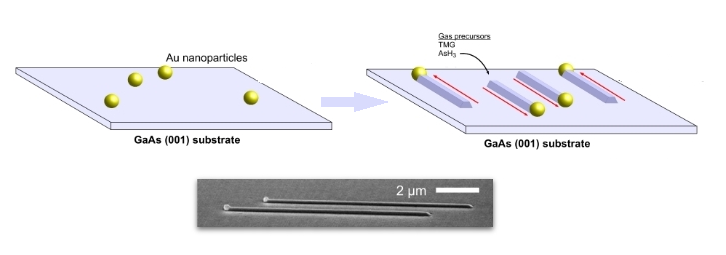
\includegraphics[width=14cm, height=5cm]{images/deposition.png} 
	\caption{Extremely thin layers bond to substrate initially}
	\label{fig:img3}  
\end{figure}
\vspace{3mm}
\newline
The molecules get adsorbed on the surface.The heat breaks up the molecules and deposits the desired atoms on the surface , layer by layer.
\vspace{3mm}
\newline
The heated organic precursor molecules decompose in the absence of oxygen (pyrolysis).Required pyrolysis temperature increases with increasing chemical bond strength of the precursor. 
\vspace{4mm}
\newline 
\begin{figure}[h!] 
	\centering
	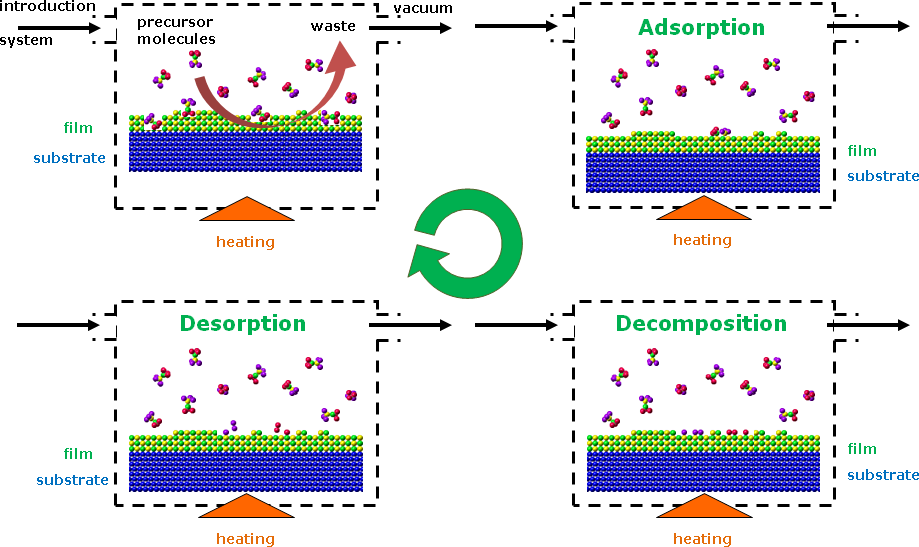
\includegraphics[width=12cm, height=9cm]{images/principles.png} 
	\caption{Overall Principle}
	\label{fig:img4} 
\end{figure}
\vspace{3mm}
\newline 
Pyrolysis leaves the atoms on the substrate surface.This is followed by desorption,a phenomenon whereby a substance is released from or through a surface.
\vspace{3mm}\newline
The atoms bond to the substrate surface and a new crystalline layer is grown in the last step. Formation of this epitaxial layer occurs at the substrate surface.
\vspace{3mm}
\newline
The undesired remnants are removed or deposited on the walls of the reactor.\newline
By varying the composition of the gas, you can change the properties of the crystal at an almost atomic scale.
\vspace{1mm}
\section{Setup required for the process}
\vspace{2mm}
In the metal organic chemical vapor deposition (MOCVD) technique, reactant gases are combined at elevated temperatures in the reactor to cause a chemical interaction, resulting in the deposition of materials on the substrate.
\vspace{3mm}
\newline
A reactor is a chamber made of a material that does not react with the chemicals being used. It must also withstand high temperatures.This chamber is composed by reactor walls, liner, a susceptor, gas injection units, and temperature control units.
\vspace{3mm}
\newline 
A susceptor is a material used for its ability to absorb electromagnetic energy and convert it to heat. A substrate sits on a susceptor which is at a controlled temperature. The susceptor is made from a material resistant to the metalorganic compounds used.
\vspace{5mm}
\newline
\begin{figure}[h!] 
	\centering
	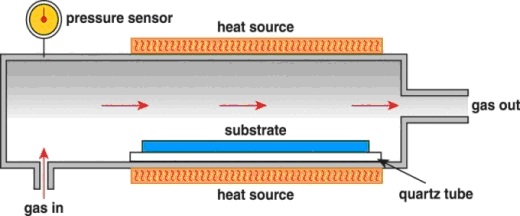
\includegraphics[width=11cm, height=5cm]{images/pyrolisis.png} 
	\caption{Heating Chamber}
	\label{fig:img5} 
\end{figure}
\vspace{3mm}
\newline 
Usually, the reactor walls are made from stainless steel or quartz.To prevent overheating, cooling water must be flowing through the channels within the reactor walls.A pressure maintenance system is also required.
\vspace{3mm}
\newline
The next component is the Gas inlet. Gas is introduced via devices known as 'bubblers'. In a bubbler a carrier gas (usually hydrogen in arsenide  phosphide growth or nitrogen for nitride growth) is bubbled through the metalorganic liquid, which picks up some metalorganic vapour and transports it to the reactor.
\vspace{3mm}
\newline
The amount of metalorganic vapour transported depends on the rate of carrier gas flow and the bubbler temperature
\vspace{3mm}
\newline
A Gas exhaust and cleaning system is also required. Toxic waste products must be converted to liquid or solid wastes for recycling (preferably) or disposal
\vspace{3mm}
\newline
\begin{figure}[h!] 
	\centering
	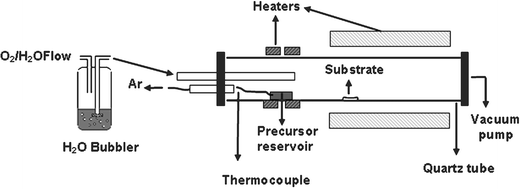
\includegraphics[width=15cm, height=10cm]{images/reactor1.png} 
	\caption{Mocvd Reactor Setup}
	\label{fig:img6} 
\end{figure}
\vspace{3mm}
\newline
Showerhead MOCVD reactors have been widely applied in recent years. They employ a perforated or porous planar surface to dispense reactant gases more-or-less uniformly over a second parallel planar surface The reactant gases are injected vertically from the showerhead flange toward the substrate.
\vspace{3mm}
\newline
The reactor built by Aixtron (Figure 1) is showerhead type.
\vspace{3mm}
\newline
Each individual wafer is located on a separate small disk, which is rotating slowly during this deposition process, providing a uniform distribution of the materials across each single wafer.
\vspace{3mm}
\newline
Along with vertical gas flow,there are also several constructions of MOCVD reactors with lateral flow.Figure 7 shows one such reactor.
\vspace{3mm}
\newline
\begin{figure}[h!] 
	\centering
	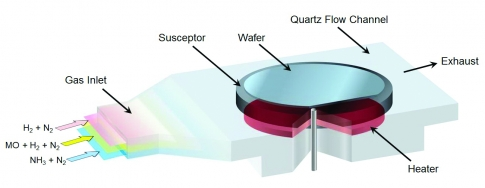
\includegraphics[width=11cm, height=5cm]{images/reactor2.png} 
	\caption{laminar flow of carrier gas (H2 or N2) and of precursor molecules (metalorganic substances) over the substrate (wafer) placed on a graphite susceptor inside a reaction vessel (reactor) }
	\label{fig:img7} 
\end{figure}
\vspace{3mm}
\newline
\section{Applications}
1. \hspace{2mm}MOCVD is used in manufacturing lasers, transistors, solar cells and other\\    \hspace{7mm}opto-electronic devices, and is the key enabling technology for future markets\\  \hspace{7mm}with high growth potential.
\vspace{5mm}
\newline
\begin{figure}[h!] 
	\centering
	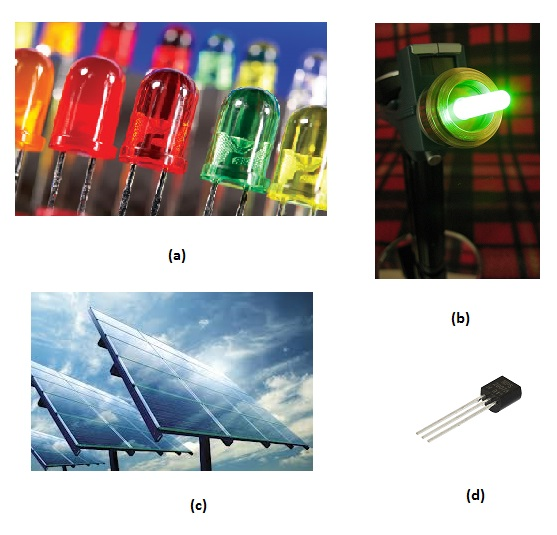
\includegraphics[width=9cm, height=8cm]{images/trans.png} 
	\caption{Applications of MOCVD-  (a)LED  (b)Laser (c)solar cell (d)transistor }
	\label{fig:img8} 
\end{figure}
\vspace{5mm}
\newline 
2. \hspace{2mm}It is used in manufacturing light-emitting diodes (LEDs).This has become the\\ \hspace{7mm}widespread standard in the private, commercial and public lighting market.This\\ \hspace{7mm}Led technology also forms an important part of LED TVs.These semiconductors\\
\hspace{7mm}are the most important base material for manufacturing red, blue, green and\\ \hspace{7mm}white LEDs.
\vspace{3mm}
\newline
3. \hspace{2mm}It is also used in the manufacturing of photodiodes and photodetectors ,though\\
\hspace{7mm}to a much lesser extent. 
\vspace{5mm}
\newline
\begin{figure}[h!] 
	\centering
	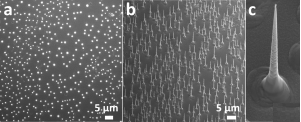
\includegraphics[width=9cm, height=4cm]{images/GaAs.png} 
	\caption{GaAs nanowire}
	\label{fig:img9} 
\end{figure}
\vspace{3mm}
\newline 
4. \hspace{2mm}It is the most significant manufacturing process for III-V compound\\ \hspace{7mm}semiconductors (eg.GaAs as shown in figure 9) of high purity, especially for\\ \hspace{7mm}those based on Gallium Nitride (GaN).It is also used for growing II-VI\\ \hspace{7mm}semiconductors such as Cadmium oxide (CdO), Zinc Sulfide (Zns) etc.
\vspace{3mm}
\newline 
5. \hspace{2mm}It is also utilized for a broad variety of applications in industry and research.
\vspace{1mm}
\section{Summary}
\vspace{2mm}
Advancements in MOCVD have always occurred in response to the requirements of the various applications of this technology .Using MOCVD we can build up many layers, each of a precisely controlled thickness, to create a material which has specific optical and electrical properties.
\vspace{3mm}\newline
Using this technique it's possible to build a range of semiconductor photodetectors and lasers, the devices that lie at the heart of the information revolution.It is expected that with time,its applications and popularity will only continue to grow.
\end{flushleft}
%\end{document}
